\documentclass{article}
\usepackage{fullpage}
\usepackage{algpseudocode}
\usepackage{tabulary}
\usepackage{algorithm}
\usepackage{graphicx}
\usepackage{multicol}
\DeclareGraphicsExtensions{.png}
\begin{document}
\begin{raggedleft}
Project 6\\
"Op" Philip Flarsheim\\
Computer Engineering \& Computer Science\\
Speed School of Engineering\\
University of Louisville, USA\\
plflar02@louisville.edu\\
\end{raggedleft}

\noindent{\Large\bf1. Introduction}

This project was an investigation in the combination of "Genetic Algorithm" and "Wisdom of Crowds" strategies to solve the Partition Sum NP complete problem. The Partition Sum problem consists of a set of $n$ integers with values ranging from $1 \to k$. These object is to determine if there are two subsets whose sums are equal. This problem was selected for investigation since its solution mapped well to the idea of a genome in Genetic Algorithms.\\

\noindent{\Large\bf2. Approach}

Genetic Algorithms take their inspiration from the biological theory of evolution. In this instance the \emph{'genome'} was defined as two lists of numbers containing numbers from the original list, with each number being used once across both lists. Each \emph{'genome'}s fitness was calculated as the difference between the sums of the two lists. The initial population was created by shuffling the array of starting integers and then splitting it at a random point into two lists. The starting population was split into several groups and were allowed to evolve in isolation for several generation; followed by a step in which randomly selected members of each population were shared with other populations. Each generation consisted of several discrete steps. First the sorted population was separated into groups each consisting of one ninth of the population and the first, third and fifth groups were taken to be the base population for the next generation. These members were then crossed at random with any of the members of the previous generation, each union resulting in two children each with a different dominant parent genome, those children were added to the new population. Second a percent chance was rolled for each member of the new population to determine if several of its genes where randomly switched. The percent chance of mutation was determined as 5\% plus 1\% for every generation in which the same member of the population was the fittest. This averaged mutation chance at about 10\%.

The Wisdom of Crowds search strategy makes use of swam intelligence by aggregating a \emph{'crowd'} and building a best solution off of each \emph{'expert's'} proposed solution. The set of experts was created by taking the top 10\% of all final solutions in the genetic algorithm. A weight system was created to consolidate the positions of each number in either the first or second list. A greedy selection method was used to build the final aggregate solution. The number of times each gene appeared in a list determined which list it was placed in for the final solution.

\begin{algorithm}
\caption{Genetic Algorithm - Main}
\begin{algorithmic}

\State $populations = randomPopulations(numPops, popSize)$
\For{$i=0 \to numIterations$}
	\ForAll{$population \in populations$}
		\State $population = EvolvePopulation(population, numGenerations)$
	\EndFor
	\State $populations = MergePopulations(populations, random.int(1, popSize/numPops), random.int(1, numPops-1))$
\EndFor
\State $Experts = populations.getTop10Percent()$
\State $Final = WisdomOfCrowds(Experts)$
\end{algorithmic}
\end{algorithm}

\begin{algorithm}
\caption{Genetic Algorithm - Evolve Population}
\begin{algorithmic}
\Function{$EvolvePopulation$}{$population, numGenerations$}
	\For{$i=0 \to numGenerations$}
		\State $newPop = population.select9nths(1,3,5)$
		\ForAll{$parent \in newPop$}
			\State $newPop.append(Crossover(parent, population.randomChoice()))$
			\State $newPop.append(Crossover(random.choice(population), parent))$
		\EndFor
		\State $population = newPop$
		\State $population.sortByFitness()$
		\State $mutateChance = leaderCount * .01 + .05$
		\ForAll{$genome \in population$}
			\If {$Random() <= mutateChance$}
				\State $Mutate(genome)$
			\EndIf
		\EndFor
		\If {$population[0] == leader$}
			\State $leaderCount++$
		\Else 
			\State $leader = population[0]$
			\State $leaderCount = 0$
		\EndIf
	\EndFor
	\State\Return $population$
\EndFunction
\end{algorithmic}
\end{algorithm}

\begin{algorithm}
\caption{Genetic Algorithm - Crossover}
\begin{algorithmic}
\Function{Crossover}{$parent1, parent2$}
	\State $child = clone(parent1)$
	\If{$parent2.list1.length > 0$}
		\For{$i=0 \to random.int(0, parent2.list1.length)$}
			\State $value = random.choice(parent2.list1)$
			\If{($child.list2.count(value) > 0)$}
				\State $child.list2.remove(value)$
				\State $child.list1.append(value)$
			\EndIf
		\EndFor
	\EndIf
	\If{$parent2.list2.length > 0$}
		\For{$i=0 \to random.int(0, parent2.list2.length)$}
			\State $value = random.choice(parent2.list2)$
			\If{($child.list1.count(value) > 0)$}
				\State $child.list1.remove(value)$
				\State $child.list2.append(value)$
			\EndIf
		\EndFor
	\EndIf
	\State\Return $child$
\EndFunction
\end{algorithmic}
\end{algorithm}

\begin{algorithm}
\caption{Genetic Algorithm - Mutate}
\begin{algorithmic}
\Function{Mutate}{$genome, numSwaps$}
	\For{$i=0 \to numSwaps$}
		\If{$random() < .5$}
			\If{($genome.list1.length > 0$}
				\State $value = random.choice(genome.list1)$
				\State $genome.list1.remove(value)$
				\State $genome.list2.append(value)$
			\EndIf
		\Else
			\If{($genome.list2.length > 0$}
				\State $value = random.choice(genome.list2)$
				\State $genome.list2.remove(value)$
				\State $genome.list1.append(value)$
			\EndIf
		\EndIf
	\EndFor
	\State\Return $genome$
\EndFunction
\end{algorithmic}
\end{algorithm}

\begin{algorithm}
\caption{Genetic Algorithm - Merge Populations}
\begin{algorithmic}
\Function{MergePopulations}{$populations, numNomads, direction$}
	\For{$i=0 \to populations.length()$}
		\For{$j=0 \to numNomads$}
			\State $nomad = random.choice(populations[i])$
			\State $populations[i].remove(nomad)$
			\State $nomads[i].append(nomad)$
		\EndFor
	\EndFor
	\For{$i=0 \to nomadss.length()$}
		\State $j = i + direction$
		\If{$j >= populations.length()$}
			\State $j -= populations.length()$
		\EndIf
		\State $populations[j].extend(nomad)$
	\EndFor
	\State\Return $populations$
\EndFunction
\end{algorithmic}
\end{algorithm}

\begin{algorithm}
\caption{Wisdom of Crowds}
\begin{algorithmic}
\Function{WisdomOfCrowds}{$baseGenome, experts$}
	\State $baseGenome.sort()$	
	\ForAll{$expert \in experts$}
		\For{$i=0 \to baseGenome.length()$}
			\If{$expert.list1.count(baseGenome[i]) > 0$}
				\State $weight1[i] += 1$
				\State $expert.list1.remove(baseGenome[i])$
			\EndIf
			
			\If{$expert.list2.count(baseGenome[i]) > 0$}
				\State $weight2[i] += 1$
				\State $expert.list2.remove(baseGenome[i])$
			\EndIf
		\EndFor
	\EndFor
	\For{$i=0 in baseGenome.length()$}
		\If{$weight1[i] > weight2[i]$}
			\State $final.list1.append(baseGenome[i])$
		\ElsIf{$weight1[i] < weight2[i]$}
			\State $final.list2.append(baseGenome[i])$
		\Else
			\If{$random() < .5$}
				\State $final.list1.append(baseGenome[i])$
			\Else
				\State $final.list2.append(baseGenome[i])$
			\EndIf
		\EndIf
	\EndFor
	\State\Return $final$
\EndFunction
\end{algorithmic}
\end{algorithm}

\newpage
\noindent{\Large\bf3. Results}

The algorithm performed significantly better than anticipated, both in speed of executed and quality of results. Several trial runs were performed in order to fine tune the algorithm's initial conditions.\\

\noindent{\large\bf3.1 Data}

The initial number set used in the trial was randomly generated by Python's Random library. Each number was an integer between the values of one and one million. The numbers used for the presented trial are presented below.

\begin{multicols}{3}

530269, 486126, 189697, 420176, 262184, 602360, 214173, 196120, 740144, 709610, 611960, 740622, 365003, 312588, 7108, 486405, 594214, 972517, 693666, 172982, 752005, 365494, 757666, 54531, 937713, 100403, 91491, 568457, 887690, 114547, 868227, 901593, 112463, 218622, 319587, 908315, 598817, 513323, 850193, 655394, 230661, 112054, 680370, 259650, 45305, 800570, 280931, 288219, 313276, 925266, 389314, 334514, 812318, 400648, 306611, 301042, 704655, 822154, 536762, 971592, 335637, 436072, 807055, 224249, 724245, 308333, 85901, 669046, 618715, 520159, 699781, 274382, 156932, 592172, 720857, 540869, 865957, 749914, 575825, 695019, 666370, 616321, 276223, 135313, 460071, 515883, 627147, 99961, 480851, 645931, 945743, 77360, 838537, 289654, 475082, 370362, 470626, 914511, 527257, 122762\\

\end{multicols}

\noindent{\large\bf3.2 Results}\\

\begin{tabulary}{\textwidth}{l L}
\hline
\bf{Initial conditions}&\\
\hline
\bf{Genome Size} & 100\\
\bf{Number of Iterations} & 25\\
\bf{Generations Per Iteration} & 100\\
\bf{Number of Populations} & 8\\
\bf{Population Size} & 250\\
\hline
\end{tabulary}\\\\

\begin{tabulary}{\textwidth}{l L}
\hline
\bf{Results}&\\
\hline
\bf{Time(s)} & 834.3586609363556\\
\bf{Sum Difference} & 2\\
\bf{List1} & 7108, 45305, 54531, 77360, 99961, 112054, 112463, 114547, 122762, 135313, 156932, 189697, 230661, 259650, 262184, 289654, 301042, 308333, 370362, 389314, 400648, 420176, 436072, 475082, 486126, 486405, 515883, 536762, 568457, 575825, 598817, 627147, 645931, 669046, 680370, 699781, 709610, 720857, 724245, 740144, 740622, 757666, 800570, 812318, 838537, 850193, 901593, 908315, 914511, 925266, 972517\\
\bf{List2} & 85901, 91491, 100403, 172982, 196120, 214173, 218622, 224249, 274382, 276223, 280931, 288219, 306611, 312588, 313276, 319587, 334514, 335637, 365003, 365494, 460071, 470626, 480851, 513323, 520159, 527257, 530269, 540869, 592172, 594214, 602360, 611960, 616321, 618715, 655394, 666370, 693666, 695019, 704655, 749914, 752005, 807055, 822154, 865957, 868227, 887690, 937713, 945743, 971592\\
\hline
\end{tabulary}

\newpage
\noindent{\large\bf3.2.1 Genetic Algorithm Results}\\
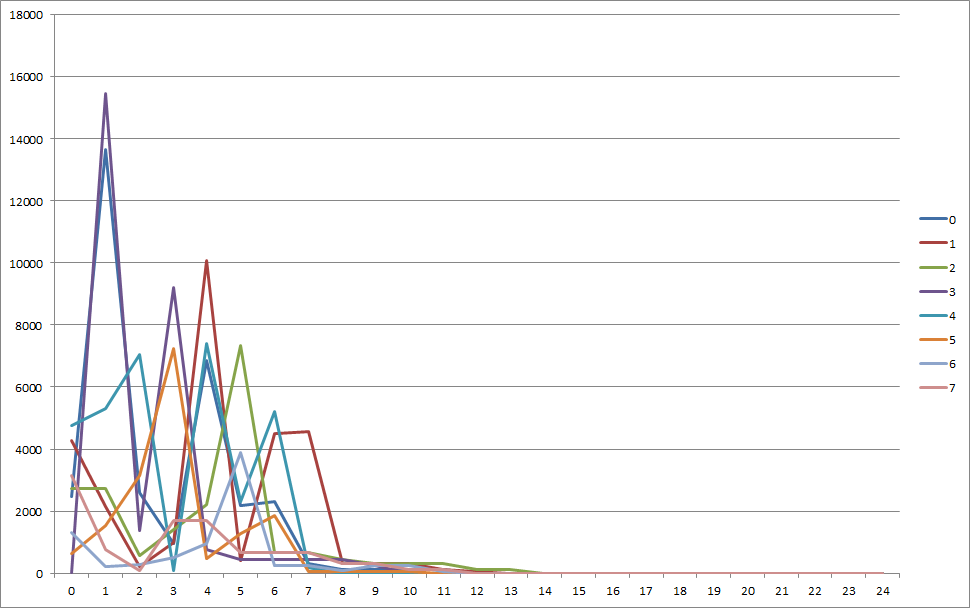
\includegraphics[width=210mm, angle=270]{results.png}

\newpage
\noindent{\large\bf3.2.2 Weight Results}\\

\begin{multicols}{3}

\begin{tabulary}{\textwidth}{|r|c|c|}
\hline
\bf{Gene} & \bf{List1} & \bf{List2}\\
\hline
7108 & 486 & 0\\
45305 & 486 & 0\\
54531 & 486 & 0\\
77360 & 486 & 0\\
85901 & 0 & 486\\
91491 & 0 & 486\\
99961 & 486 & 0\\
100403 & 0 & 486\\
112054 & 486 & 0\\
112463 & 486 & 0\\
114547 & 486 & 0\\
122762 & 486 & 0\\
135313 & 486 & 0\\
156932 & 486 & 0\\
172982 & 0 & 486\\
189697 & 486 & 0\\
196120 & 0 & 486\\
214173 & 0 & 486\\
218622 & 0 & 486\\
224249 & 0 & 486\\
230661 & 486 & 0\\
259650 & 486 & 0\\
262184 & 486 & 0\\
274382 & 0 & 486\\
276223 & 0 & 486\\
280931 & 0 & 486\\
288219 & 0 & 486\\
289654 & 486 & 0\\
301042 & 486 & 0\\
306611 & 0 & 486\\
308333 & 486 & 0\\
312588 & 0 & 486\\
313276 & 0 & 486\\
319587 & 0 & 486\\
\hline
\end{tabulary}

\begin{tabulary}{\textwidth}{|r|c|c|}
\hline
\bf{Gene} & \bf{List1} & \bf{List2}\\
\hline
334514 & 0 & 486\\
335637 & 0 & 486\\
365003 & 0 & 486\\
365494 & 0 & 486\\
370362 & 486 & 0\\
389314 & 486 & 0\\
400648 & 486 & 0\\
420176 & 486 & 0\\
436072 & 486 & 0\\
460071 & 0 & 486\\
470626 & 0 & 486\\
475082 & 486 & 0\\
480851 & 0 & 486\\
486126 & 486 & 0\\
486405 & 486 & 0\\
513323 & 0 & 486\\
515883 & 486 & 0\\
520159 & 0 & 486\\
527257 & 0 & 486\\
530269 & 0 & 486\\
536762 & 486 & 0\\
540869 & 0 & 486\\
568457 & 486 & 0\\
575825 & 486 & 0\\
592172 & 0 & 486\\
594214 & 0 & 486\\
598817 & 486 & 0\\
602360 & 0 & 486\\
611960 & 0 & 486\\
616321 & 0 & 486\\
618715 & 0 & 486\\
627147 & 486 & 0\\
645931 & 486 & 0\\
655394 & 0 & 486\\
\hline
\end{tabulary}

\begin{tabulary}{\textwidth}{|r|c|c|}
\hline
\bf{Gene} & \bf{List1} & \bf{List2}\\
\hline
666370 & 0 & 486\\
669046 & 486 & 0\\
680370 & 486 & 0\\
693666 & 0 & 486\\
695019 & 0 & 486\\
699781 & 486 & 0\\
704655 & 0 & 486\\
709610 & 486 & 0\\
720857 & 486 & 0\\
724245 & 486 & 0\\
740144 & 486 & 0\\
740622 & 486 & 0\\
749914 & 0 & 486\\
752005 & 0 & 486\\
757666 & 486 & 0\\
800570 & 486 & 0\\
807055 & 0 & 486\\
812318 & 486 & 0\\
822154 & 0 & 486\\
838537 & 486 & 0\\
850193 & 486 & 0\\
865957 & 0 & 486\\
868227 & 0 & 486\\
887690 & 0 & 486\\
901593 & 486 & 0\\
908315 & 486 & 0\\
914511 & 486 & 0\\
925266 & 486 & 0\\
937713 & 0 & 486\\
945743 & 0 & 486\\
971592 & 0 & 486\\
972517 & 486 & 0\\
\hline
\end{tabulary}

\end{multicols}

\newpage
\noindent{\Large\bf4. Discussion}

The algorithm performed better than expected in both execution time and in quality of results. Genetic algorithms lend themselves significantly better to the Partition Sum problem since the genome does not need to be balanced. This allowed for for effective crossover and faster execution time. Additionally the implementation of isolated populations allowed the algorithm to try multiple paths concurrently. Unfortunately in many of the trial runs the Genetic algorithm was able to calculate the best solution without the need for aggregation through the Wisdom of Crowds algorithm.\\

\noindent{\Large\bf5. References}

The matplotlib library was used to render the data set and to provide a UI in which to inspect the results. Documentation can be found at http://matplotlib.sourceforge.net/.
\end{document}